%% Version 4.3.2, 25 August 2014
%
%%%%%%%%%%%%%%%%%%%%%%%%%%%%%%%%%%%%%%%%%%%%%%%%%%%%%%%%%%%%%%%%%%%%%%
% Template.tex --  LaTeX-based template for submissions to the 
% American Meteorological Society
%
% Template developed by Amy Hendrickson, 2013, TeXnology Inc., 
% amyh@texnology.com, http://www.texnology.com
% following earlier work by Brian Papa, American Meteorological Society
%
% Email questions to latex@ametsoc.org.
%
%%%%%%%%%%%%%%%%%%%%%%%%%%%%%%%%%%%%%%%%%%%%%%%%%%%%%%%%%%%%%%%%%%%%%
% PREAMBLE
%%%%%%%%%%%%%%%%%%%%%%%%%%%%%%%%%%%%%%%%%%%%%%%%%%%%%%%%%%%%%%%%%%%%%

%% Start with one of the following:
% DOUBLE-SPACED VERSION FOR SUBMISSION TO THE AMS
\documentclass{ametsoc}

% TWO-COLUMN JOURNAL PAGE LAYOUT---FOR AUTHOR USE ONLY
%\documentclass[twocol]{ametsoc}

%%%%%%%%%%%%%%%%%%%%%%%%%%%%%%%%
%%% To be entered only if twocol option is used

\journal{mwr}

%  Please choose a journal abbreviation to use above from the following list:
% 
%   jamc     (Journal of Applied Meteorology and Climatology)
%   jtech     (Journal of Atmospheric and Oceanic Technology)
%   jhm      (Journal of Hydrometeorology)
%   jpo     (Journal of Physical Oceanography)
%   jas      (Journal of Atmospheric Sciences)	
%   jcli      (Journal of Climate)
%   mwr      (Monthly Weather Review)
%   wcas      (Weather, Climate, and Society)
%   waf       (Weather and Forecasting)
%   bams (Bulletin of the American Meteorological Society)
%   ei    (Earth Interactions)

%%%%%%%%%%%%%%%%%%%%%%%%%%%%%%%%
%Citations should be of the form ``author year''  not ``author, year''
\bibpunct{(}{)}{;}{a}{}{,}

%%%%%%%%%%%%%%%%%%%%%%%%%%%%%%%%

%%% To be entered by author:

%% May use \\ to break lines in title:

\title{Physics-dynamics coupling with element-based high-order Galerkin methods: quasi equal-area physics grid}

%%% Enter authors' names, as you see in this example:
%%% Use \correspondingauthor{} and \thanks{Current Affiliation:...}
%%% immediately following the appropriate author.
%%%
%%% Note that the \correspondingauthor{} command is NECESSARY.
%%% The \thanks{} commands are OPTIONAL.

    %\authors{Author One\correspondingauthor{Author One, 
    % American Meteorological Society, 
    % 45 Beacon St., Boston, MA 02108.}
% and Author Two\thanks{Current affiliation: American Meteorological Society, 
    % 45 Beacon St., Boston, MA 02108.}}

\authors{Adam R. Herrington\correspondingauthor{Adam R. Herrington, School of Marine and Atmospheric Sciences, Stony Brook University, Stony Brook, New York, USA.}}

%% Follow this form:
    % \affiliation{American Meteorological Society, 
    % Boston, Massachusetts.}

\affiliation{School of Marine and Atmospheric Sciences, Stony Brook University, Stony Brook, New York, USA.}

%% Follow this form:
    %\email{latex@ametsoc.org}

\email{adam.herrington@stonybrook.edu}

%% If appropriate, add additional authors, different affiliations:
\extraauthor{Peter H. Lauritzen}
\extraaffil{Climate and Global Dynamics, National Center for Atmospheric Research, 1850 Table Mesa Drive, Boulder, Colorado, USA.}
\extraauthor{Mark A. Taylor}
\extraaffil{Sandia National Laboratories, Albuquerque, New Mexico, USA.}
\extraauthor{Steve Goldhaber, Brian E. Eaton and Julio T. Bacmeister}
\extraaffil{Climate and Global Dynamics, National Center for Atmospheric Research, 1850 Table Mesa Drive, Boulder, Colorado, USA.}
\extraauthor{Kevin A. Reed}
\extraaffil{School of Marine and Atmospheric Sciences, Stony Brook University, State University of New York, Stony Brook, New York.}
\extraauthor{Paul A. Ullrich}
\extraaffil{Department of Land, Air and Water Resources, University of California, Davis, California, USA.}

%% May repeat for a additional authors/affiliations:

%\extraauthor{}
%\extraaffil{}

%%%%%%%%%%%%%%%%%%%%%%%%%%%%%%%%%%%%%%%%%%%%%%%%%%%%%%%%%%%%%%%%%%%%%
% ABSTRACT
%
% Enter your abstract here
% Abstracts should not exceed 250 words in length!
%
% For BAMS authors only: If your article requires a Capsule Summary, please place the capsule text at the end of your abstract
% and identify it as the capsule. Example: This is the end of the abstract. (Capsule Summary) This is the capsule summary. 

\abstract{Atmospheric modeling with element-based high-order Galerkin methods presents a unique challenge to the conventional physics-dynamics coupling paradigm, due to the highly irregular distribution of nodes within an element and the distinct numerical characteristics of the Galerkin method. The conventional coupling procedure is to evaluate the physical parameterizations ({\em{physics}}) on the dynamical core grid. Evaluating the physics at the nodal points exacerbates numerical noise from the Galerkin method, enabling and amplifying local extrema at element boundaries. Grid imprinting may be substantially reduced through the introduction of an entirely separate, approximately isotropic finite-volume grid for evaluating the physics forcing. Integration of the spectral basis over the control-volumes provides an area average state to the physics, which is more representative of the state in the vicinity of the nodal points rather than the nodal point itself, and is more consistent with the notion of a `large-scale state' required by conventional physics packages. This study documents the implementation of a quasi-equal area physics grid into NCAR's Community Atmosphere Model with Spectral Elements, and is shown to be effective at mitigating grid imprinting in the solution. The physics grid is also appropriate for coupling to other components within the Community Earth System Model, since the coupler requires component fluxes to be defined on a finite-volume grid, and one can be certain that the fluxes on the physics grid are indeed, volume-averaged.}

\begin{document}

%% Necessary!
\maketitle


%%%%%%%%%%%%%%%%%%%%%%%%%%%%%%%%%%%%%%%%%%%%%%%%%%%%%%%%%%%%%%%%%%%%%
% MAIN BODY OF PAPER
%%%%%%%%%%%%%%%%%%%%%%%%%%%%%%%%%%%%%%%%%%%%%%%%%%%%%%%%%%%%%%%%%%%%%
%

%% In all cases, if there is only one entry of this type within
%% the higher level heading, use the star form: 
%%
\section{Introduction}
An increasing number of numerical methods publications in the atmospheric science literature concern transport, shallow-water, and three-dimensional models employing element-based high-order Galerkin discretizations such as finite-element and discontinuous Galerkin methods \citep[for an introduction to these methods see, e.g., ][]{Durran,NLL2011LNCSE,U2014GMD}. Some global models based on Galerkin methods have reached a level of maturity for which they are being considered for next generation climate and weather models due to their inherent conservation properties, high-order accuracy (for smooth problems), high parallel efficiency, high processor efficiency, and geometric flexibility facilitating mesh-refinement applications. NCAR's Community Atmosphere Model \citep[CAM; ][]{CAM5} offers a dynamical core based on continuous Galerkin finite elements \citep{TF2010JCP}, referred to as CAM-SE \citep[CAM Spectral Elements; ][]{TES2008JPCS,DetAl2012IJHPCA,LetAl2018JAMES}. CAM-SE is, in particular, being used for high resolution climate modeling \citep[e.g., ][]{JAME:JAME20125,RetAl2015GRL,BETAL2018CC} and static mesh-refinement applications \citep[e.g., ][]{FT2004MWR,ZetAl2014JC,ZetAl2014JCb,GetAl2014GMD,RHUZ2016JAMC}. Other examples of models based on high-order Galerkin methods that are being considered for `operational' weather-climate applications are \citet{Giraldo20083849}, \citet{NCT2009CF}, \citet{BSBDK2013TCFD} and the Energy Exascale Earth System Model (\url{https://e3sm.org/}).

%\begin{figure}[t]
\begin{figure*}[t]
\begin{center}
\noindent\includegraphics[width=37pc,angle=0]{gll.pdf}\\
%\noindent\includegraphics[width=15pc,angle=0]{figs/quadrature-fig/gll.pdf}\\
%\noindent\includegraphics[width=37pc,angle=0]{figs/quadrature-fig/gll.pdf}\\
\end{center}
\noindent
\caption{Example of CAM-SE GLL quadrature grids, marked with red filled circles, (a \& c) on the cubed-sphere and (b \& d) in an element. (a)-(b) and (c)-(d) use $4\times 4$ ($np=4$) and $8\times 8$ ($np=8$) GLL quadrature points in each element, respectively. (a) and (c) have the same average grid-spacing at the Equator (7.5$^\circ$) which is obtained by using (a) $4\times 4$ ($ne=4$) and (b) $2\times 2$ ($ne=2$) elements on each cubed-sphere face/panel, respectively. The element boundaries are marked with thick light blue lines. The grid configurations shown on (a) and (c) are referred to as $ne4np4$ and $ne2np8$, respectively.}
\label{fig:gll-grids}
%\end{figure}
\end{figure*}

Assumptions inherent to the physical parameterizations (also referred to as {\em{physics}}) require the state passed by the dynamical core represent a `large-scale state', for example, in quasi-equilibrium-type convection schemes \citep{AS1974JAS,PC2008JAS}. In finite-volume methods \citep[e.g., ][]{L2004MWR}, one may think of the dynamical core state as the average state of the atmosphere over a control volume, and for resolutions typical of climate simulations is entirely consistent with the notion of a `large-scale state'. For finite-difference methods \citep[e.g., ][]{SETAL983MWR} the point value is thought of as representative for the atmospheric state in the vicinity of the point value and one can usually associate a volume with the grid-point. Hence the physics grid (the grid on which the state of the atmosphere is evaluated and passed to physics) and the dynamics grid (the grid the dynamical core uses) coincide. Having the physics and dynamics grids coincide is obviously convenient since no interpolation is needed (which could disrupt conservation properties) and the number of degrees of freedom on both grids is exactly the same. 

For the regular latitude-longitude, cubed-sphere and icosahedral grids the distance between the grid-points is gradually varying for finite-volume/finite-difference discretizations. Examples of models that use these grids are CAM-FV \citep[latitude-longitude grid, ][]{L2004MWR}, FV3 \citep[cubed-sphere grid, ][]{PL2007JCP} and ICON \citep[icosahedral grid, ][]{WETAL2013GMD}. For high-order element-based Galerkin methods, the dynamical core grid is defined by the quadrature points. In CAM-SE, these are the Gauss-Lobatto-Legendre (GLL) quadrature nodes. A unique aspect of the high-order quadrature rules is that the nodes within an element are located at the roots of the basis set, which may be irregularly spaced. For example, Figure \ref{fig:gll-grids} shows GLL points on an individual element of a cubed-sphere grid for degree 3 ($np\times np=4\times 4$ quadrature points) and degree 7 ($np\times np=8\times 8$ quadrature points) Lagrange polynomial basis used in CAM-SE. The higher the order of the quadrature rule, the greater variance in distance between GLL quadrature points within an element. GLL quadrature points cluster near the edges and, in particular, the corners of the elements.

The resolved scales of motion are not determined by the distance between quadrature nodes, but rather the degree of the polynomial basis in each element. The nodes may be viewed as irregularly spaced samples of an underlying spectrally truncated state. From this perspective, one might expect the nodal solutions to be independent of location within an element. While the interior quadrature nodes are $C^{\infty}$ in CAM-SE (i.e. the basis representation is infinitely smooth and all derivatives are continuous), the smoothness of boundary nodes are constrained by the need to patch neighboring solutions together to form the global basis set, an operation known as the direct stiffness summation \citep[DSS; ][]{MadayPatera87,canuto2007}. The DSS operation is attractive because it allows for high-order accuracy with minimal communication between elements, but degrades the solution to $C^0$ at element boundaries (i.e., all derivatives are discontinuous). Through evaluating the physics at the nodal points, strong grid-scale forcing or oscillatory behavior near an element boundary may exacerbate the discontinuity, and our initial expectation, that the nodal solutions are independent of within-element location, is unlikely for non-smooth problems, e.g., the presence of rough topography or moist physics grid-scale forcing.

It is the purpose of this paper to document the implementation of an entirely separate, quasi-equal area finite-volume physics grid into CAM-SE. The use of a separate physics grid is not entirely unheard of; prior studies have utilized the infrastructure developed for global-spectral transform methods to experiment with different physics grids \citep{W1999T,W2014PTRSL}. In our framework, the dynamical core state is integrated over control volumes to provide a volume averaged state to the physics, thereby minimizing the influence of any one particular nodal value on the physics forcing. Section \ref{sec:nodeproblem} provides a thorough explanation of how grid imprinting manifests in high-order Galerkin methods for non-smooth problems. The implementation of the physics grid configuration into CAM-SE is presented in Section \ref{sec:methods}. Results from a hierarchy of idealized model configurations are presented in Section \ref{sec:results}, illustrating the physics grid is effective at mitigating undesirable grid imprinting in the solution. Section \ref{sec:conclusions} contains a discussion of results and concluding remarks.

\section{The Quadrature Node Problem}\label{sec:nodeproblem}

Figure~\ref{fig:se-schematic} is a schematic illustrating in one-dimension how grid-imprinting is enabled by the physics, when the dynamical core is built using high-order Galerkin methods. The schematic depicts a time-step, starting from smooth initial conditions (Figure~\ref{fig:se-schematic}a), and subsequently advancing the dynamics one Runge-Kutta time-step (Figure~\ref{fig:se-schematic}b). Since the boundary nodes of adjacent elements overlap one-another, there are now two solutions for each boundary node. The DSS operator, effectively a numerical flux applied to the element boundaries such that overlapping nodal values agree, is applied (Figure~\ref{fig:se-schematic}c), rendering the solutions at element boundaries $C^0$; less-smooth than neighboring $C^{\infty}$ interior nodes. An element boundary discontinuity may be exacerbated if, e.g., the physics updates the state at an element boundary (Figure~\ref{fig:se-schematic}d,e), resulting in characteristically tighter gradients on the boundary nodes compared to if the physics forcing were applied to an interior node (Figure~\ref{fig:se-schematic}g,h).   

\begin{figure*}[t]
\noindent\includegraphics[width=38pc,angle=0]{se-schematic-arh-CROP.pdf}\\
%\noindent\includegraphics[width=38pc,angle=0]{figs/se-schematic-arh-CROP.pdf}\\
\caption{A one-dimensional schematic showing the relationship between the basis functions, the quadrature nodes and the proposed physics grid, over the coarse of a time-step. The filled circles are the GLL quadrature points in each element, which are connected by a Lagrange polynomials basis (curves). (a) Smooth initial condition are (b) advanced by the dynamics one Runge-Kutta step (blue), and (c) shows the solution after applying the DSS operator. Applying (d) grid-scale forcing to an element boundary node, (e) the basis representation is clearly $C^0$ at the element boundary. In contrast, (d) applying grid-scale forcing to an interior node (e) results in a smooth, $C^{\infty}$ continuous field. (f),(i) Vertical bars pertain to the values on the physics grid, found through integrating the basis functions over the control volumes.}
\label{fig:se-schematic}
\end{figure*}

To test the degree to which nodal solutions depend on within-element position, an aqua-planet simulation \citep{NH2000ASL,MWO2016JAMES}, which consists of an ocean covered planet in perpetual equinox, with fixed, zonally symmetric sea surface temperatures idealized after the present day climatology, is carried out using CAM-SE, using CAM, version 4 physics \citep[CAM4;][]{CAM4} and run for one year. The nominal low resolution $ne30np4$ grid is used, pertaining to an average equatorial grid spacing of $111.2km$. The probability density distribution of the upward vertical pressure velocity ($\omega$), conditionally sampled based on three categories - `interior', `edge' and `corner' nodes - is provided in Figure~\ref{fig:omega-se-volumes}a. The motivation for assessing noise in the $\omega$ field comes from its connection with the atmosphere's divergent modes, as follows from the continuity equation in pressure coordinates. These modes are in turn sensitive to the within-element inhomogeneity of the pressure gradient that emerges from high-order Galerkin methods. There is an apparent dependence on nodal location, with interior nodes being characteristically sluggish, and corner and edge nodes having systematically larger magnitude vertical motion. This behavior is consistent with the smoothness properties of the different nodal locations, with discontinuous pressure gradients resulting in greater vertical motion at edge and corner nodes. The main division of solutions shown in Figure~\ref{fig:omega-se-volumes}a is primarily between whether a node is, or is not situated on an element boundary, and is a nuanced signature of high-order element-based Galerkin methods for non-smooth problems.

\begin{figure*}[t]
\begin{center}
\noindent\includegraphics[width=37pc,angle=0]{temp_pdf_200bins_30min_trX25min.pdf}\\
%\noindent\includegraphics[width=18pc,angle=0]{figs/temp_pdf_200bins_30min_trX25min.pdf}\\
%\noindent\includegraphics[width=37pc,angle=0]{figs/temp_pdf_200bins_30min_trX25min.pdf}\\
\end{center}
\caption{Probability density distribution of instantaneous upward $\omega$ in a pair of aqua-planet simulations using CAM4 physics. Figure is constructed from one year of six hourly data, at all vertical levels. (a) $ne30np4$ configuration conditionally sampled for interior, edge and corner node control volumes, and similarly (b) for the $ne30pg3$ configuration. {\color{red}{The curves in (b) are overlain in (a) in grey, and similarly the curves in (a) are overlain in (b).}} Note the consistently larger magnitude $\omega$ for boundary nodes compared with interior nodes in (a), and that the bias is substantially reduced through mapping to a quasi-equal area physics grid.}\label{fig:omega-se-volumes}
\end{figure*}

If the conventional physics-dynamics coupling paradigm is applied to CAM-SE, then the physics are to be evaluated at the GLL nodes, and a volume associated with the quadrature point should be defined. One approach to construct this grid is to decompose each spectral element into $(np-1) \times (np-1)$ subcells and then take the dual grid of this subcell grid.  For cubed-sphere meshes, this dual grid will have a control volume associated with each quadrature point. These control volumes will be triangles for the cube corner quadrature points and quadrilaterals for all remaining quadrature points.  Newton iteration can than be used to adjust the corners of these control volumes so that their spherical area exactly match the Gaussian weight multiplied by the metric term (these weights are used for integrating the basis functions over the elements and can therefore, in this context, be interpreted as areas).  For cubed-sphere meshes, the Newton iteration can be replaced by a direct method if some of the quadrilaterals are replaced by pentagons giving additional flexibility in matching the spherical area to the quadrature weights. Such a dual grid is shown in Figure \ref{fig:cv-grids}. This grid is used in the NCAR CESM (Community Earth System Model) coupler for passing states between ocean, atmosphere and land components since the current remapping method is finite-volume based and therefore requires control volumes (it is noted that methods exist that do not require control volumes for conservative interpolation, e.g., \cite{UT2015MWR}). Hence the components `see' an irregular atmospheric grid. Similarly, the parameterizations in the atmosphere `see' a state that is anisotropically sampled in space \citep[see Figure 1 and 5 in ][]{KetAl2008JGR}.

%\begin{figure}[t]
\begin{figure*}[t]
\begin{center}
\noindent\includegraphics[width=37pc,angle=0]{se_gll_cv_grid.eps}\\
%\noindent\includegraphics[width=15pc,angle=0]{figs/se_gll_cv_grid.eps}\\
%\noindent\includegraphics[width=37pc,angle=0]{figs/se_gll_cv_grid.eps}\\
\end{center}
\caption{An example of control volumes constructed around GLL quadrature points ($ne4np4$) so that the spherical area of the control volumes exactly match the quadrature weight multiplied by the metric factor.}
\label{fig:cv-grids}
%\end{figure}
\end{figure*}


The quadrature grid in element-based Galerkin methods is defined to perform mathematical operations on the basis functions, e.g., computing gradients and integrals, rather than evaluating the state variables for physics-dynamics coupling. One may argue that it would be more consistent to integrate the basis functions over quasi-equal area control volumes within each element and pass those control volume average values to physics rather than irregularly spaced quadrature point values. In this case when integrating basis functions over control volumes a grid-cell average value is more representative of the values near the extrema at the element boundary than the quadrature point value. The relationship between the nodal values, the basis functions and the proposed control volumes is illustrated schematically in one-dimension in parts (f) and (i) in Figure~\ref{fig:se-schematic}. 

\section{Methods}\label{sec:methods}
Here we focus on CAM-SE, however, in principle the methods apply to any element-based high-order Galerkin model. The physics grid in CAM-SE is defined by sub-dividing each element using equi-angular gnomonic coordinate lines to define the sides of the physics grid control volumes (see the Appendix for details). Note that the element boundaries are defined by equi-angular gnomonic grid lines. The notation $pg=3$ refers to the configuration where the elements are divided into $pg\times pg=3\times 3$ equi-angular physics grid cells (see Figure \ref{fig:np4_pg3}) resulting in a quasi-equal spherical area grid resembling the cubed-sphere. Defining the physics grid by sub-dividing elements makes it possible to use the same element infrastructure as already used in CAM-SE, thereby facilitating its implementation. Here we make use of the $ne30np4$ and $ne30pg3$ grids that use GLL quadrature point physics grid (physics and dynamics grid coincide), and the same ($pg=3$) resolution quasi equal-area physics grids, respectively. In all configurations we use degree three Lagrange basis ($np=4$) and $ne\times ne=30\times 30$ elements on each cubed-sphere panel.

%\begin{figure}[t]
\begin{figure*}[t]
\begin{center}
\noindent\includegraphics[width=37pc,angle=0]{np4_pg3.pdf}\\
%\noindent\includegraphics[width=15pc,angle=0]{figs/np4_pg3.pdf}\\
%\noindent\includegraphics[width=37pc,angle=0]{figs/np4_pg3.pdf}\\
\end{center}
\caption{A schematic illustration of an element, indicating the relationship between (left) the dynamical core grid, and (right) the proposed quasi-equal area physics grid. The physics grid contains $pg\times pg=3\times 3$ grid cells in each element.}
\label{fig:np4_pg3}
%\end{figure}
\end{figure*}

A consequence of separating physics and dynamics grids is that the atmospheric state must be mapped to the physics grid and the physics tendencies must be mapped back to the dynamics grid. This is discussed in separate sections below. When separating physics and dynamics grids it is advantageous to use a vertical coordinate that is static during physics-dynamics coupling. This was one motivation to switch to a dry-mass vertical coordinate in CAM-SE \citep{LetAl2018JAMES}; since dry mass remains constant throughout physics the dry-mass vertical coordinate remains fixed during physics-dynamics coupling. The dry mass coordinate subsequently evolves as floating Lagrangian layers by the dynamics \citep{L2004MWR} periodically mapped back to a reference hybrid-sigma-pressure coordinate after \cite{SB1981MWR}. All variables mapped between grids are collocated, layer-mean values \citep{LetAl2018JAMES}.
 
\subsection{Mapping state from dynamics grid (GLL) to physics grid (pg)}
The dynamics state is defined on the GLL grid in terms of temperature $T^{(gll)}$, zonal wind component $u^{(gll)}$, meridional wind component $v^{(gll)}$, and dry pressure level thickness $\Delta p^{(gll)}$. In the mapping of the atmospheric state to the physics grid it is important that the following properties are met:
\begin{enumerate}
\item conservation of scalar quantities such as mass and dry thermal energy,\label{prop1}
\item for tracers; shape-preservation (monotonicity), i.e., the mapping method must not introduce new extrema in the interpolated field, in particular, negatives,\label{prop2}
\item consistency, i.e., the mapping preserves a constant,\label{prop3}
\item linear correlation preservation{\color{red}{, i.e., if field $A$ is a linear function of $B$, this relationship is still preserved \citep[see, e.g, equation 5 in][]{LT2011QJR}}}
\end{enumerate}
Other properties that may be important, but not pursued here, includes total energy conservation and axial angular momentum conservation. Total energy is a quadratic quantity that is inherently difficult to conserve unless one maps total energy requiring one to diagnose either temperature or momentum components. For example, enforcing total energy conservation locally using, e.g., \citet{L2004MWR}'s method where total energy and velocity components are remapped and temperature is a derived variable, has proven problematic (C. Chen, personal communication). Similarly conservation of axial angular momentum is problematic. Conservation of angular momentum requires one to interpolate the zonal and meridional components of momentum which creates large errors near the poles. To avoid the pole problem we interpolate contra-variant components of the momentum vector, which violates axial angular momentum conservation.

We argue that the most consistent method for mapping scalar state variables from the GLL grid to the physics grid is to integrate the Lagrange basis function representation (used by the SE dynamical core) over the physics grid control volumes, i.e., integrate the basis function representation of $\Delta p^{(gll)}\times T^{(gll)}$ and $\Delta p^{(gll)}$ over the physics grid control volume \citep[see, e.g., ][]{LTOUNGK2017MWR,UT2015MWR}
\begin{eqnarray}
\Delta p^{(pg)}&=&\frac{1}{A^{(pg)}}\int_{A^{(pg)}}\Delta p^{(gll)}\, dA,\\
T^{(pg)}&=&\frac{}{A^{(pg)}\Delta p^{(pg)}}\int_{A^{(pg)}}T^{(gll)}\Delta p^{(gll)}\, dA,
\end{eqnarray}
where $A^{(pg)}$ is the physics grid area. The integrals are numerically computed using the GLL quadrature rule on each physics grid element, which exactly (to machine precision) integrates the basis functions over the $pg$ control volumes \citep{LTOUNGK2017MWR}. Thermal energy and dry air mass is conserved and the mapping is consistent. For the wind, which is a vector, the zonal and meridional wind components are mapped by transforming to contra-variant wind components, evaluating the basis function representation thereof at the equi-angular center of the physics grid control volumes and then transformed back to latitude-longitude coordinate system winds. All of the operations are local to the element and do not require communication between elements.

The mapping of tracers is more problematic since the SE basis function representation is oscillatory although the shape-preserving filter guarantees shape-preservation at the GLL nodes \citep{GTS2014JCP}. To avoid this issue we use the CAM-SE-CSLAM version of CAM-SE \citep[Conservative Semi-Lagrangian Multi-tracer transport scheme][]{LTOUNGK2017MWR}, where tracers are advected on the $pg=3$ physics grid using the inherently mass and linear-correlation preserving CSLAM algorithm. Note that in CAM-SE-CSLAM the dry mass internally predicted by CSLAM, $\Delta p^{(cslam)}$, is, by design, equal to $\Delta p^{(gll)}$ integrated over the CSLAM/physics grid control volume \citep{LTOUNGK2017MWR}. Since the tracer grid and physics grids are co-located and $\Delta p^{(pg)}=\Delta p^{(cslam)}$ then the  mass conservation, correlation preservation, consistency and shape-preservation constraints are inherently fulfilled.
%
\subsection{Mapping tendencies from physics grid (pg) to dynamics grid (GLL)}
The physics tendencies are computed on the finite-volume physics grid and are denoted $f_T^{(pg)}$,$f_u^{(pg)}$,$f_v^{(pg)}$, and $f_m^{(pg)}$. Note that dry air mass is not modified by physics and hence there is no tendency for dry mass,  $f_{\Delta p}\equiv 0$. Also, it is important to map tendencies and not state from the physics grid to GLL grid otherwise one will get spurious tendencies from mapping errors when the actual physics tendency is zero (unless a reversible map is used).

It is important that this process:
\begin{enumerate}
\item for tracers; mass tendency is conserved,
\item for tracers; in each tracer grid cell the mass tendency from physics must not exceed tracer mass available in tracer grid cell (it is assumed that the physics tendency will not drive tracer mixing ratio negative on the physics grid),\label{item:phys2fvm_consistency}
\item linear correlation preservation,
\item consistency, i.e., the mapping preserves a constant tendency.
\end{enumerate}
Other properties that may be important, but not pursued here, includes total energy conservation (incl. components of total energy) and axial angular momentum conservation. Scalar variables are mapped from the physics grid to GLL grid using a tensor-product Lagrange interpolation in two dimensions (i.e., we assume that the pressure variations in the vertical are small). The local coordinates on a cubed-sphere are discontinuous at the element edges so the interpolation requires special attention at the cube corners and edges. The details are provided in the Appendix. Lagrange interpolation preserves a constant (including zero) and linear correlations. Tracer and physics grids are co-located so tracer mass, tracer shape, and tracer correlations are trivially preserved on the tracer grid; and the inconsistency in point \ref{item:phys2fvm_consistency} above will not appear. 

Mapping from $pg$ to GLL grids while conserving mass was found to be difficult without excessive grid imprinting at element edges. Mass-conservation (using conventional finite-volume methods) requires a control volume to be defined around the GLL points \cite[see Figure \ref{fig:cv-grids} in this paper or Figure 8b in ][]{UDJ2016MWR}. These volumes are artificial and not consistent with the SE method. Integrating the CSLAM reconstruction of water tracers of such artificial control volumes led to GLL node grid imprinting in the mapping and will not preserve a constant mixing ratio since the mapping of $\Delta p^{(pg)}$ to GLL will not yield the GLL node value for dry pressure-level thickness (i.e., the maps are not reversible).  A reversible map requires that the number of degrees of freedom on the source mesh ($pg3$ has 9 degrees of freedom) equal the number of degrees of freedom on the target mesh ($np4$ grid has 16 degrees of freedom). This condition is violated by construction for individual elements.

It was also found important to use an interpolator that is smooth across element boundaries. Using an algorithm that only uses information from an element of control volumes will (at best) be $C^0$ at the element boundaries and therefore lead to boundary node grid imprinting. A stencil that extends beyond one element is therefore necessary. After much experimentation, the best results in terms of grid-imprinting were obtained with tensor-cubic interpolation (see the Appendix for details) and by using the CAM-SE-CSLAM configuration (which requires the same boundary exchange/communication as used in CSLAM).

\subsection{Time splitting and physics-dynamics coupling}

The physics and dynamics are integrated in time using a sequential-update approach \citep[e.g.,][]{W2002MWR}. The dynamical core is sub-cycled over the (usually) longer physics time-step, $\Delta t_{phys}$, e.g., the vertical remapping time-step $\Delta t_{remap}$ is cycled {\color{red}{$nsplit$}} times, totaling to $\Delta t_{phys}$. In CAM-SE, a fraction of the physics forcing, e.g., $f_q \times \Delta t_{remap}$ is applied at the beginning of each {\color{red}{$nsplit$}} vertical remap subcycles, such that the full forcing ($f_q \times \Delta t_{phys}$) is realized over the course of a physics time-step. This approach of dribbling the tendencies over sub-intervals has the advantage of reducing gravity wave noise \citep{TJ2016GMD}, but may disrupt tracer mass conservation \citep{water-leak}. In CAM-SE-CSLAM, all but the tracer mass quantities are dribbled, with tracer mass receiving the full physics update, e.g., $f_q \times \Delta t_{phys}$, applied only at the beginning of the first remap sub-cycle, and thereby conserving tracer mass. This is the $ftype=2$ configuration described in detail in Section 3.6.3 in \cite{LetAl2018JAMES}.

In the SE integration of the equations of motion on the GLL grid the water species are needed in the computation of the pressure gradient force and generalized expressions for heat capacity at constant pressure $c_p$, etc. Hence the mixing ratios for water vapor and dynamically/thermodynamically active condensates (e.g., cloud liquid and cloud ice) are needed on the GLL grid. We have chosen to advect the water species on the GLL grid using the SE method as well as on the physics grid using CSLAM. Every time physics updates the water species on the CSLAM grid, a forcing term (equal to the difference between updated CSLAM water variables and the SE values) is applied to the GLL water variables using dribbling so that the CSLAM solution and SE solution for water species are tightly coupled. 

\section{Results}\label{sec:results}

A hierarchy of idealized model configurations are presented in order to elucidate the differences between CAM-SE and CAM-SE-CSLAM (available from the CESM2.1 release; \url{https://doi.org/10.5065/D67H1H0V}). Here, the configurations are presented in order of increasing complexity, each with a pair of approximately $1^{\circ}$ simulations, pertaining to the $ne30np4$ (CAM-SE) and $ne30pg3$ (CAM-SE-CSLAM) grids, and a $\Delta t_{phys}$ = 1800 s.

\subsection{Moist Baroclinic Wave}

The moist baroclinic wave test case was developed as part of the `CESM Simple Models' project \citep{CESM_SIMPLER_MODELS}, and included in the release of CESM2. It is effectively the dry test-case of \cite{UMJS2014QJRMS}, but initialized with moisture and coupled to the Kessler moist physics routine \citep{K1969MM}. For more details on this test case \cite[which was part of the 2016 Dynamical Core Model Intercomparison Project, ][]{DCMIP16}, see Section 4.1 in \cite{LetAl2018JAMES}. A measure of the uncertainty in the reference solution, the $L_2$ difference norm between two high-resolution solutions using different dynamical cores, was also presented in \cite{LetAl2018JAMES} and provided again here in Figure \ref{fig:norm}. The $L_2$ norm between CAM-SE and CAM-SE-CSLAM lies below the uncertainty of the reference solution, indicating their differences are insignificant.

%\begin{figure}[t]
\begin{figure*}[t]
\begin{center}
%\noindent\includegraphics[width=15pc,angle=0]{figs/temp_l2.pdf}\\
%\noindent\includegraphics[width=37pc,angle=0]{figs/temp_l2.pdf}\\
\noindent\includegraphics[width=37pc,angle=0]{temp_l2.pdf}\\
\end{center}
\caption{$L_2$ difference norms of the surface pressure field, $p_s$, in the moist baroclinic wave simulations. $L_2$ values lying within the yellow region fall below the estimate of the uncertainty in the reference solution (black curve), computed as the difference norm between two approximately $0.25^\circ$ resolution versions of CAM, the spectral-element and finite-volume (CAM-FV) dynamical cores.}
\label{fig:norm}
%\end{figure}
\end{figure*}

The flow field of the baroclinic wave test is used to drive the terminator ``toy"-chemistry test of \cite{LCLVT2015GMD,LTOUNGK2017MWR}. The terminator test is used to assess linear-correlation preservation using two reactive species advected across the terminator line. The model is initialized with species for which their weighted sum, $Cl_y$, is a constant (constant surface pressure and constant mixing ratio;$\ Cl_y = Cl + 2Cl_2 = 4\times 10^{-6}\ kg/kg$), such that if tracer correlations are preserved, then the column-integrated weighted sum of the species should not vary in time. Figure \ref{fig:term} provides a snapshot of the vertically integrated weighted sum of species at day 15. In CAM-SE, the tracer correlations are not preserved at day 15 and the field is populated by overshoots and undershoots. In contrast, by day 15, CAM-SE-CSLAM still conserves tracer correlations to within machine precision, consistent with the previous results of this test-case initialized with a dry baroclinic wave \citep{LTOUNGK2017MWR}. 

%\begin{figure}[t]
\begin{figure*}[t]
\begin{center}
%\noindent\includegraphics[width=15pc,angle=0]{figs/terminator_iCLy.pdf}\\
%\noindent\includegraphics[width=37pc,angle=0]{figs/terminator_iCLy.pdf}\\
\noindent\includegraphics[width=37pc,angle=0]{terminator_iCLy.pdf}\\
\end{center}
\caption{Results of the terminator ``toy"-chemistry test. Snapshot of the total column integrated, weighted sum of the species,$\ \left< Cl_y \right> = \left< Cl \right> + \left< 2Cl_2 \right>$, in kg/kg, at day 15 of the moist baroclinic wave test. (Top) CAM-SE, (Bottom) CAM-SE-CSLAM.}
\label{fig:term}
%\end{figure}
\end{figure*}

\subsection{Aqua-planets}

Two year long aqua-planet simulations are performed using CAM-SE and CAM-SE-CSLAM, using the CAM4 physics package \citep{CAM4}, as discussed in Section \ref{sec:nodeproblem}. Away from the grid-scale, the mean states in the two models are very similar. Figure~\ref{fig:zonal} shows the zonal-mean climatological precipitation rates in CAM-SE and CAM-SE-CSLAM. Considering how sensitive this aqua-planet configuration is to design choices in CAM-SE \citep{LetAl2018JAMES}, it is somewhat unexpected that the zonal means look so similar to one another. 

%\begin{figure}[t]
\begin{figure*}[t]
\begin{center}
%\noindent\includegraphics[width=15pc,angle=0]{figs/temp_dzonal.pdf}\\
%\noindent\includegraphics[width=37pc,angle=0]{figs/temp_dzonal.pdf}\\
\noindent\includegraphics[width=37pc,angle=0]{temp_dzonal.pdf}\\
\end{center}
\caption{Climatological zonal-mean total precipitation rate in the aqua-planets, computed from a pair of year long simulations.}
\label{fig:zonal}
%\end{figure}
\end{figure*}

A plot similar to Figure \ref{fig:omega-se-volumes}a is constructed for the CAM-SE-CSLAM simulation, a probability density distribution of upward $\omega$ conditionally sampled based on location within the element. Like Figure \ref{fig:omega-se-volumes}a, Figure \ref{fig:omega-se-volumes}b divides up the control volumes by corner, edge and interior cells. Through the use of the quasi-equal area physics grid, the dynamical core state appears more or less independent of location within the element, a marked improvement over CAM-SE. Since the state is approximately independent of in-element location, it follows that the physics forcing, which is evaluated from the dynamical core state, may be expected to also show an improvement in grid-imprinting. 

The low-level, mean and variance of the temperature tendencies from the physics, on the GLL grid, $f_T^{(gll)}$, in the two simulations are shown in Figure \ref{fig:tendency_imprint}. The mean states in the two models resemble one another, consistent with the zonal mean precipitation rates (Figure~\ref{fig:zonal}). The mean physics tendencies contains modest grid imprinting in CAM-SE (barely visible near the storm-track regions), while in the variance field, grid imprinting is both ubiquitous and unmistakable. The variance is larger on boundary nodes, manifesting as a `stitching' pattern resembling the cube-sphere grid. In CAM-SE-CSLAM, the grid imprinting is all but eliminated based on the mean and variance of the physics tendencies (Figure~\ref{fig:tendency_imprint}), consistent with our expectation.

{\color{red}{The global mean and variance of the low-level physics tendencies are marginally lower in CAM-SE-CSLAM compared with CAM-SE on the GLL grid (by about 1\% and 6\% for the mean and variance, respectively; Figure~\ref{fig:tendency_imprint}). While these differences may be small, and potentially insignificant, they are consistent with the state on the GLL grid in the two simulations. Through re-creating Figure \ref{fig:omega-se-volumes}a, but using the $\omega$ field on the GLL grid in the CAM-SE-CSLAM run, the frequency of large magnitude $\omega$ values (less than -1.0 Pa/s) associated with interior, corner and edge nodes is slightly lower (not shown). This suggests that the lower magnitude physics forcing in CAM-SE-CSLAM impacts the state on the GLL grid, albeit modestly. Therefore the lower frequency of large magnitude $\omega$ in CAM-SE-CSLAM (Figure \ref{fig:omega-se-volumes}) may not be solely due to the smoothing effect of integrating the basis functions over control volumes, but also the lower magnitude physics tendencies feeding back onto the dynamical state.}}

As stated in Section \ref{sec:methods}, the mapping of the state to the physics grid and the reverse interpolation of physics tendencies to the GLL grid is not total energy conserving. CAM has a global energy fixer \citep{WOHTTV2015JAMES} which can be used to estimate the errors associated with the mapping algorithms. To do so, it is presumed that there are no compensating mapping errors in going to and from the physics and dynamics grids, and that CAM-SE-CSLAM and CAM-SE have the same energy dissipation rates. Under these assumptions the spurious globally integrated total energy errors due to the mapping algorithm is estimated to be approximately 0.0025 $W/m^2$ in the aqua-planet simulations. In comparison, the dynamical core total energy dissipation is on the order of 0.1 $W/m^2$ \citep{LetAl2018JAMES}. 

\begin{figure*}[t]
\noindent\includegraphics[width=37pc,angle=0]{QPC4_bar_skk.pdf}\\
%\noindent\includegraphics[width=19pc,angle=0]{figs/QPC4_bar_skk.pdf}\\
%\noindent\includegraphics[width=37pc,angle=0]{figs/QPC4_bar_skk.pdf}\\
\caption{Mean (left) and variance (right) of the low level temperature tendencies from the physical parameterizations on the GLL grid, with the $ne30np4$ configuration, (top row) and $ne30pg3$ configuration (bottom row), in a pair of year-long aqua-planet simulations. Grid imprinting is observed along the element boundaries in $ne30np4$, but is absent from the $ne30pg3$ simulation.}
\label{fig:tendency_imprint}
\end{figure*}

\subsection{Held-Suarez with Topography}

Grid imprinting associated with the flow around obstacles is more problematic than that encountered on the aqua-planets. In order to diagnose grid imprinting due to topographic flow, an idealized Held-Suarez configuration \citep{HS1994} is outfitted with real world topography after \cite{FRETAL2000WMR,BETAL2006MWR}, and run for two years. Figure~\ref{fig:FHS-contours} shows the mean $\omega$ at two different vertical levels in the middle troposphere. {The data are presented as a raster plot on their respective unstructured grids, in order to delineate whether a particular value is associated with an interior, edge or element boundary node. 

At higher latitudes (e.g., the southern Andes), the flow is smooth, conforming reasonably to the underlying topography. At lower latitudes, over the Andes ({\color{red}{between the equator and $20^{\circ}S$}}) or the Himalayas ({\color{red}{from $20^{\circ}N$ to $30^{\circ}N$}}), there is a clear preference for extrema to occur at the element boundaries (Figure~\ref{fig:FHS-contours}). The vertical structure of $\omega$ in regions of strong grid-imprinting indicates full-troposphere upward/downward motion (not shown). Grid imprinting is therefore more common in regions of weak stratification, such as occurs in the deep tropics, with forced up-slope flow facilitating the release of gravitational instability. Resolved updrafts/downdrafts often align with the element boundaries due to its systematically tighter pressure gradients. 

\begin{figure*}[t]
%\noindent\includegraphics[width=37pc,angle=0]{FHS-contours-CROP.pdf}\\
\noindent\includegraphics[width=37pc,angle=0]{figs/FHS-contours-CROP.pdf}\\
\caption{Mean $\omega$ at two model levels in the middle troposphere, in a Held-Suarez configuration outfitted with real world topography. (Left) CAM-SE state on the GLL grid, $ne30np4$, (Middle) CAM-SE-CSLAM state on the physics grid, $ne30pg3$ and (Right) {\color{red}{their differences computed through bi-linear interpolation to a common latitude-longitude grid.}} The $\omega$ fields are computed from a 1200 day Held-Suarez simulation. The data are contoured according to a `cell fill' approach, in which the coupler grids (e.g, Figure~\ref{fig:cv-grids}) are used to delineate the vertices of the control volumes.}
\label{fig:FHS-contours}
\end{figure*}

Through the use of the quasi-equal area physics grid, grid imprinting due to topographic flow is reduced (Figures~\ref{fig:FHS-contours}). The native topography lives on the physics grid, and the topography is mapped to the nodal points at run-time in CAM-SE-CSLAM. Mapping topography to the quadrature nodes ensures that no new extrema will be introduced to the boundary nodes, where the solution is least smooth. This effect can not be very large, since grid noise over topography is similar in CAM-SE and CAM-SE-CSLAM on the GLL grid {\color{red}{(not shown)}}. From the perspective of the physics grid, CAM-SE-CSLAM clearly mitigates the influence of grid-induced extrema on the state. {\color{red}{This can be seen by comparing Figures~\ref{fig:FHS-contours}a and 10b, and their differences (Figure~\ref{fig:FHS-contours}c)}, which shows that the largest differences coincide with the element boundaries}. The reduction in grid imprinting in this modified Held-Suarez configuration appears to be almost entirely a result of the smoothing effect of integrating the basis functions over the control volumes of the physics grid.

\subsection{AMIP type simulations}

A pair of 20 year-long AMIP type simulations are performed, using CAM, version 6 physics package (CAM6) and using perpetual year 2000 SST boundary conditions ($F2000climo$ compset in CESM2.0; \url{https://doi.org/10.5065/D67H1H0V}). Figure~\ref{fig:AMIP-region} shows the climatological precipitation fields in CAM-SE (left) and CAM-SE-CSLAM (middle), and over the same mountainous regions as in Figure~\ref{fig:FHS-contours}. The plots have some similar features to the $\omega$ field in the Held-Suarez runs; the greater variance at lower latitudes, and on the windward side of the mountains are broadly similar. CAM-SE-CSLAM has a lower spatial variance, e.g., the lack of extrema over the Andes at about $15^\circ$ S compared to CAM-SE, and the grid-scale precipitation peak over the Himalayas at about $30^\circ$ N. The difference plot (Figure~\ref{fig:AMIP-region}; right panel) is more broadly populated by blue, purple and white contours, indicating that CAM-SE has, in general, larger magnitude precipitation rates over high topography. The difference plots also highlight a couple of zonally aligned strips of anomalous precipitation, in particular, near the foot of the Himalayas in CAM-SE. These bands are in the same location as the bands of precipitation identified in CAM-SE in \cite{gmdd-8-4623-2015} (their Figure 7), but using CAM, version 5 physics, of which they argue are spurious in nature. 

\begin{figure*}[t]
\noindent\includegraphics[width=37pc,angle=0]{AMIP_regional.pdf}\\
%\noindent\includegraphics[width=37pc,angle=0]{figs/AMIP_regional.pdf}\\
\caption{Climatological total precipitation rate (in mm/day) computed from the final 19 years of a pair of 20 year long AMIP type simulations. (Left) CAM-SE, (middle) CAM-SE-CSLAM and (Right) their differences.}
\label{fig:AMIP-region}
\end{figure*}

To assist in identifying whether a particular precipitation pattern is spurious, an $F2000climo$ simulation is carried out using the finite-volume dynamical core that uses a regular latitude-longitude $0.9^{\circ}\times 1.25^\circ$ grid \citep[CAM-FV; $f09$ grid; ][]{CAM5}. CAM-FV is the default low resolution model in CESM2.0, and with its smoothly varying grid, does not suffer from the Quadrature Node Problem (Section \ref{sec:nodeproblem}). Figure~\ref{fig:AMIP-global} shows the global precipitation fields in CAM-SE, CAM-SE-CSLAM and CAM-FV, compared to an observational dataset, the Global Precipitation Climatology Project (GPCP; 1979-2003) gridded dataset \citep{H2001JH}. The magnitude of the precipitation rates in all three models are higher than the GPCP dataset, primarily over land in the Tropics (note the lack of red contours in the GPCP dataset), which should be interpreted cautiously due to widely-accepted issues in constructing a reliable, gridded, global precipitation dataset. At lower latitudes, CAM-FV has lower spatial variance, and overall lower magnitudes, compared with CAM-SE. The GPCP dataset indicates that perhaps the precipitation rates in low-latitude mountainous regions in CAM-FV and CAM-SE are larger than in reality. Following suit, the reduction in magnitude and spatial variance in precipitation in these regions in CAM-SE-CSLAM may be interpreted as an improvement over CAM-SE.

\begin{figure}[t]
%\begin{figure*}[t]
\begin{center}
%\noindent\includegraphics[width=18pc,angle=0]{figs/AMIP_global.pdf}\\
%\noindent\includegraphics[width=20pc,angle=0]{figs/AMIP_global.pdf}\\
\noindent\includegraphics[width=20pc,angle=0]{AMIP_global.pdf}\\
\end{center}
\caption{Climatological total precipitation rate computed from the final 19 years of a suite of 20 year long AMIP simulations, using CAM-SE (ne30np4), CAM-SE-CSLAM (ne30pg3) and CAM-FV (f09). The top plot is an observational product, the gridded GPCP climatological precipitation dataset.}
\label{fig:AMIP-global}
\end{figure}
%\end{figure*}

\section{Conclusions}\label{sec:conclusions}

Element-based high-order Galerkin Methods possess many of the attractive qualities recommended for next generation global atmospheric models. Among these, high-order accuracy is achieved with minimal communication between elements, allowing for near perfect scaling on massively parallel systems. Element communication amounts to a numerical flux applied to the element boundaries, reconciling overlapping solutions of adjacent elements but degrading the smoothness of the boundary nodes in the process (to $C^0$). For non-smooth problems, gradients are systematically tighter at the element boundaries, and local extrema often characterize the boundary nodes. This behavior is illustrated using NCAR's Community Atmosphere Model with Spectral Elements dynamics (CAM-SE) in an aqua-planet configuration, in a Held-Suarez configuration with real-world topography and in an AMIP type configuration.

The authors argue that the conventional physics-dynamics coupling paradigm, in which the physical parameterizations are evaluated on the dynamical core grid, exacerbates grid imprinting. A separate physics grid is proposed and implemented in CAM-SE, and referred to as CAM-SE-CSLAM, through dividing the elements into quasi-equal areas with equivalent degrees of freedom. The state is mapped to the physics grid with high-order accuracy through integrating CAM-SE's Lagrange basis functions over the control volumes. Control volumes near element boundaries now represent a state in the vicinity of the extrema produced through the boundary exchange, as opposed to the the nodal value itself. These control volumes are also compatible with a `large-scale state' as required by the physical parameterizations. The physical parameterizations are evaluated on the finite volume grid, and the forcing terms are mapped back to the dynamical core grid using a cubic tensor-product Lagrange interpolation. In aqua-planet simulations, evaluating the parameterizations on the physics grid removes any obvious dependence of proximity to the element boundary, resulting in a more realistic state with negligible grid imprinting. The mapping algorithm does not conserve total energy, but it is estimated that these errors are one to two orders of magnitude less than the total energy dissipation from the dynamical core.

In CAM-SE-CSLAM, the physics grid replaces the default CAM-SE quadrature point-based coupler grid (Figure~\ref{fig:cv-grids}) to compute fluxes between model components in the Community Earth System Model (CESM). The appeal here is two-fold. Through integrating the Lagrange basis functions over control volumes, one can be certain that the fluxes computed from this grid are a volume averaged flux. The same can not be said for CAM-SE, where artificial control volumes (with sizes proportional quadrature weights) are constructed around nodal values and assumed to represent the volume averaged state. The second advantage of the new coupler grid is that extrema occurring on boundary nodes may no longer influence other model components in simulations without rough topography. While grid imprinting is effectively eliminated in the aqua-planets, experiments with real-world topography (Held-Suarez and AMIP type configurations) reduces, but does not entirely eliminate, imprinting from the mean state. The quasi-equal area physics grid is nonetheless effective at mitigating numerical nuances associated with high-order element-based Galerkin methods, for non-smooth problems. 

Future work will focus on the impact of using a coarser, $pg\times pg=2\times 2$ physics grid configuration. The coarser physics grid may be more effective at reducing spurious noise over regions of rough topography, while potentially reducing the computational overhead. Any advantages of using a coarser resolution physics grid will be weighed against any potential reduction in a model's effective resolution.

%%%%%%%%%%%%%%%%%%%%%%%%%%%%%%%%%%%%%%%%%%%%%%%%%%%%%%%%%%%%%%%%%%%%%
% ACKNOWLEDGMENTS
%%%%%%%%%%%%%%%%%%%%%%%%%%%%%%%%%%%%%%%%%%%%%%%%%%%%%%%%%%%%%%%%%%%%%
%
\acknowledgments
NCAR is sponsored by the National Science Foundation (NSF). We thank three anonymous reviewers for their helpful comments that significantly improved the clarity of the manuscript. Herrington thanks NCAR's Computational and Information Systems Laboratory (CISL) and NCAR's Climate and Global Dynamics division (CGD) for computational resources and technical support. Herrington, Reed, and Lauritzen are grateful to the NCAR Advanced Study Program graduate visitor program for funding Herrington's 12-month visit. Goldhaber was partially supported by the Accelerated Climate Modeling for Energy (ACME) project, and work package $12-015334$ ``Multiscale Methods for Accurate, Efficient, and the Accelerated Scale-Aware Models, both funded through the U.S. Department of Energy Office of Biological and Environmental Research. Goldhaber is also partially supported through NSF award AGS-$1500187$ ``Development and Testing of a Global Quasi 3-D multi Modeling Framework." Model source code is officially released with CESM2.1 (\url{https://doi.org/10.5065/D67H1H0V}).

%%%%%%%%%%%%%%%%%%%%%%%%%%%%%%%%%%%%%%%%%%%%%%%%%%%%%%%%%%%%%%%%%%%%%
% APPENDIXES
%%%%%%%%%%%%%%%%%%%%%%%%%%%%%%%%%%%%%%%%%%%%%%%%%%%%%%%%%%%%%%%%%%%%%
%
% Use \appendix if there is only one appendix.
\appendix
The mapping of the physics tendencies from the physics grid to the GLL grid is done with tensor-cubic Lagrange interpolation. The elements of the cubed-sphere in SE are created from an equi-angular gnomonic projection. Consider one element $(\alpha,\beta) \in \left[ \alpha^{(elem)}_1,\alpha^{(elem)}_2 \right]\times \left[ \beta^{(elem)}_1,\beta^{(elem)}_2\right]$, where $(\alpha,\beta)$ are central angle coordinates and $\alpha^{(elem)}_1$ and $\alpha^{(elem)}_2$ are the minimum and maximum central angles in the $\alpha$-coordinate direction, respectively, and similarly for $\beta$. Let $\Delta \alpha^{(elem)}=\alpha^{(elem)}_2-\alpha^{(elem)}_1$ and $\Delta \beta^{(elem)}=\beta^{(elem)}_2-\beta^{(elem)}_1$. The physics grid cell central angle centers are located at
\begin{multline}
(\alpha^{(pg)}_i,\beta^{(pg)}_j)= \Big[ \alpha^{(elem)}_1+\left(i-\tfrac{1}{2}\right) \Delta \alpha^{(pg)},\\
                                      \beta^{(elem)}_1+\left(j-\tfrac{1}{2}\right) \Delta \beta^{(pg)}\Big],
\end{multline}
where $\Delta \alpha^{(pg)}=\Delta \beta^{(pg)}=\frac{\Delta \alpha^{(elem)}}{pg}=\frac{\Delta \beta^{(elem)}}{pg}$. The interpolation is performed in central-angle coordinates using tensor product cubic interpolation. For elements located on a cubed-sphere edge or corner the coordinate system for neighboring elements may be on a different panel. To take into account this coordinate change the central angle locations of physics grid cell centers located on other panels are transformed to the coordinate system of the panel the element in question is located on \cite[the transformations are given in, e.g.,  ][]{NTL2005MWRb}. An illustration is given in Figure \ref{fig:mapping} for an element located in the lower left corner of a panel. The element in question is $(\xi,\chi)\in (-1,1)^2$ where, for simplicity, we have transformed the element coordinates into normalized coordinates $(\xi,\chi) = \left( \frac{ 2\left(\alpha^{(pg)}-\alpha^{(elem)}_1\right)}{\Delta \alpha^{(elem)}}-1,\frac{2\left( \beta^{(pg)}-\beta^{(elem)}_1\right)}{\Delta \beta^{(elem)}}-1\right)$; also used internally in the SE dynamical core \citep[see, e.g., section 3.3 in ][]{LetAl2018JAMES}. The GLL points are located at -1,$-1/\sqrt{1}$, $1/\sqrt{5}$, and 1 in each coordinate direction. Near the edges/corners of an element cubic extrapolation is used if the centered stencil expands beyond the panel.

%\begin{figure}[t]
\begin{figure*}[t]
\begin{center}
\noindent\includegraphics[width=37pc,angle=0]{mapping.pdf}\\
%\noindent\includegraphics[width=20pc,angle=0]{figs/mapping/mapping.pdf}\\
\end{center}
\caption{Schematic of the coordinate system in which the dimensionally split cubic Lagrange interpolation is computed.  The physics grid centers are marked with asterisks and the GLL points, we are interpolating to, with solid filled circles. The element in which the GLL points are located is  bounded by  thick black lines and located in the lower left corner of a panel. The stippled lines mark the boundaries of the remaining elements. For simplicity we are using the normalized coordinate centered at the element on which the GLL points we are interpolating to are located. Note that the coordinates for points on neighboring panels (using a different local coordinate system) must be transformed to the coordinate system of the element in question.}
\label{fig:mapping}
%\end{figure}
\end{figure*}

%\appendix

% Use \appendix[A], \appendix}[B], if you have multiple appendixes.
%\appendix[A]

%% Appendix title is necessary! For appendix title:
%\appendixtitle{}

%%% Appendix section numbering (note, skip \section and begin with \subsection)
% \subsection{First primary heading}

% \subsubsection{First secondary heading}

% \paragraph{First tertiary heading}

%% Important!
%\appendcaption{<appendix letter and number>}{<caption>} 
%must be used for figures and tables in appendixes, e.g.,
%
%\begin{figure}
%\noindent\includegraphics[width=19pc,angle=0]{figure01.pdf}\\
%\appendcaption{A1}{Caption here.}
%\end{figure}
%
% All appendix figures/tables should be placed in order AFTER the main figures/tables, i.e., tables, appendix tables, figures, appendix figures.
%
%%%%%%%%%%%%%%%%%%%%%%%%%%%%%%%%%%%%%%%%%%%%%%%%%%%%%%%%%%%%%%%%%%%%%
% REFERENCES
%%%%%%%%%%%%%%%%%%%%%%%%%%%%%%%%%%%%%%%%%%%%%%%%%%%%%%%%%%%%%%%%%%%%%
% Make your BibTeX bibliography by using these commands:
\bibliographystyle{ametsoc2014}
\bibliography{bib}


%%%%%%%%%%%%%%%%%%%%%%%%%%%%%%%%%%%%%%%%%%%%%%%%%%%%%%%%%%%%%%%%%%%%%
% TABLES
%%%%%%%%%%%%%%%%%%%%%%%%%%%%%%%%%%%%%%%%%%%%%%%%%%%%%%%%%%%%%%%%%%%%%
%% Enter tables at the end of the document, before figures.
%%
%
%\begin{table}[t]
%\caption{This is a sample table caption and table layout.  Enter as many tables as
%  necessary at the end of your manuscript. Table from Lorenz (1963).}\label{t1}
%\begin{center}
%\begin{tabular}{ccccrrcrc}
%\hline\hline
%$N$ & $X$ & $Y$ & $Z$\\
%\hline
% 0000 & 0000 & 0010 & 0000 \\
% 0005 & 0004 & 0012 & 0000 \\
% 0010 & 0009 & 0020 & 0000 \\
% 0015 & 0016 & 0036 & 0002 \\
% 0020 & 0030 & 0066 & 0007 \\
% 0025 & 0054 & 0115 & 0024 \\
%\hline
%\end{tabular}
%\end{center}
%\end{table}

%%%%%%%%%%%%%%%%%%%%%%%%%%%%%%%%%%%%%%%%%%%%%%%%%%%%%%%%%%%%%%%%%%%%%
% FIGURES
%%%%%%%%%%%%%%%%%%%%%%%%%%%%%%%%%%%%%%%%%%%%%%%%%%%%%%%%%%%%%%%%%%%%%
%% Enter figures at the end of the document, after tables.
%%
%
%\begin{figure}[t]
%  \noindent\includegraphics[width=19pc,angle=0]{figure01.pdf}\\
%  \caption{Enter the caption for your figure here.  Repeat as
%  necessary for each of your figures. Figure from \protect\cite{Knutti2008}.}\label{f1}
%\end{figure}

\end{document}
